\chapter{Introduction}
\label{cha:introduzione}
Looking up at a clear night sky, we are faced with one of the most majestic spectacles nature has to offer: the starry sky.
\begin{figure}[H]
	\centering
	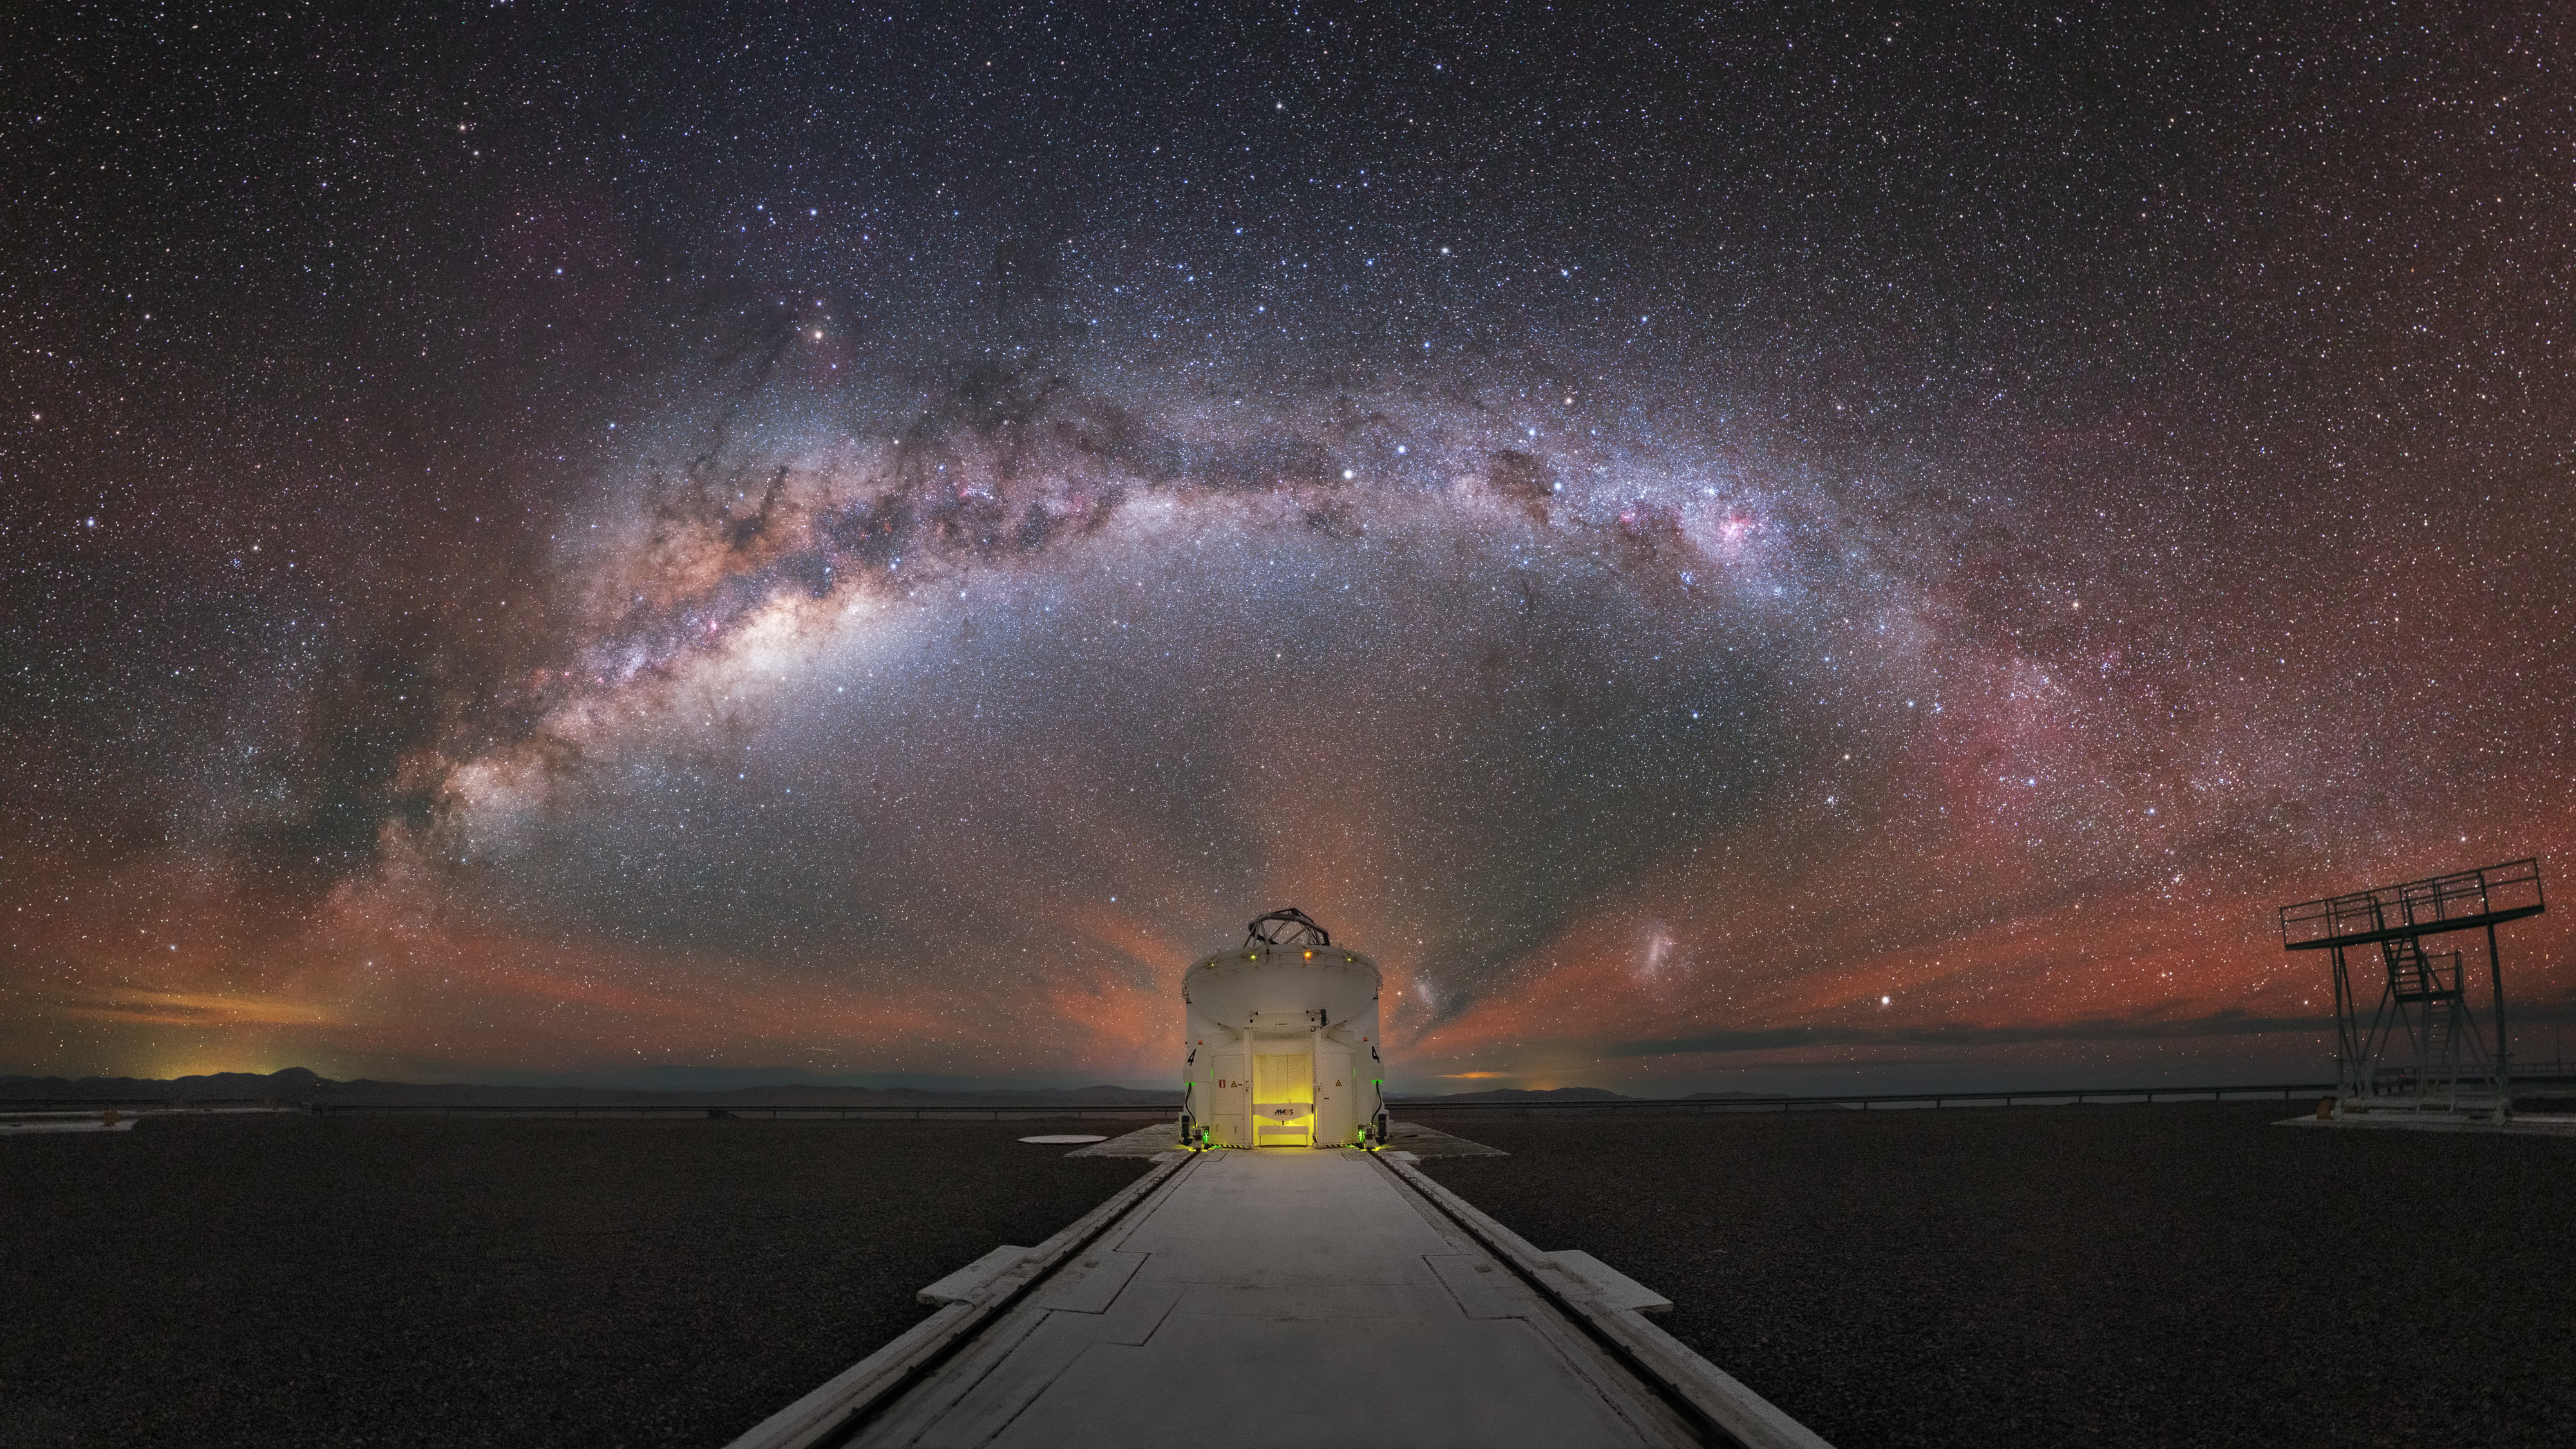
\includegraphics[width=0.60\textwidth]{./images/volto-stellato.jpg}
	\caption{The starry sky above the Paranal Observatory in Chile (Credits: R. Wesson/ESO).}
	\label{fig:volta-celeste}
\end{figure}
\noindent The starry sky presents an image of a seemingly motionless universe, in which stars appear as fixed points of light, separated by distances that are difficult to imagine. In reality, what we observe is merely a snapshot of a constantly evolving cosmos. In interstellar space, immense concentrations of gas and dust, known as nebulae, can collapse under the influence of gravity, giving birth to new stars. On even larger scales, the same force helps organise matter into increasingly complex structures, from planetary systems to entire galaxies.
\begin{figure}[H]
	\centering
	\makebox[\textwidth][c]{
		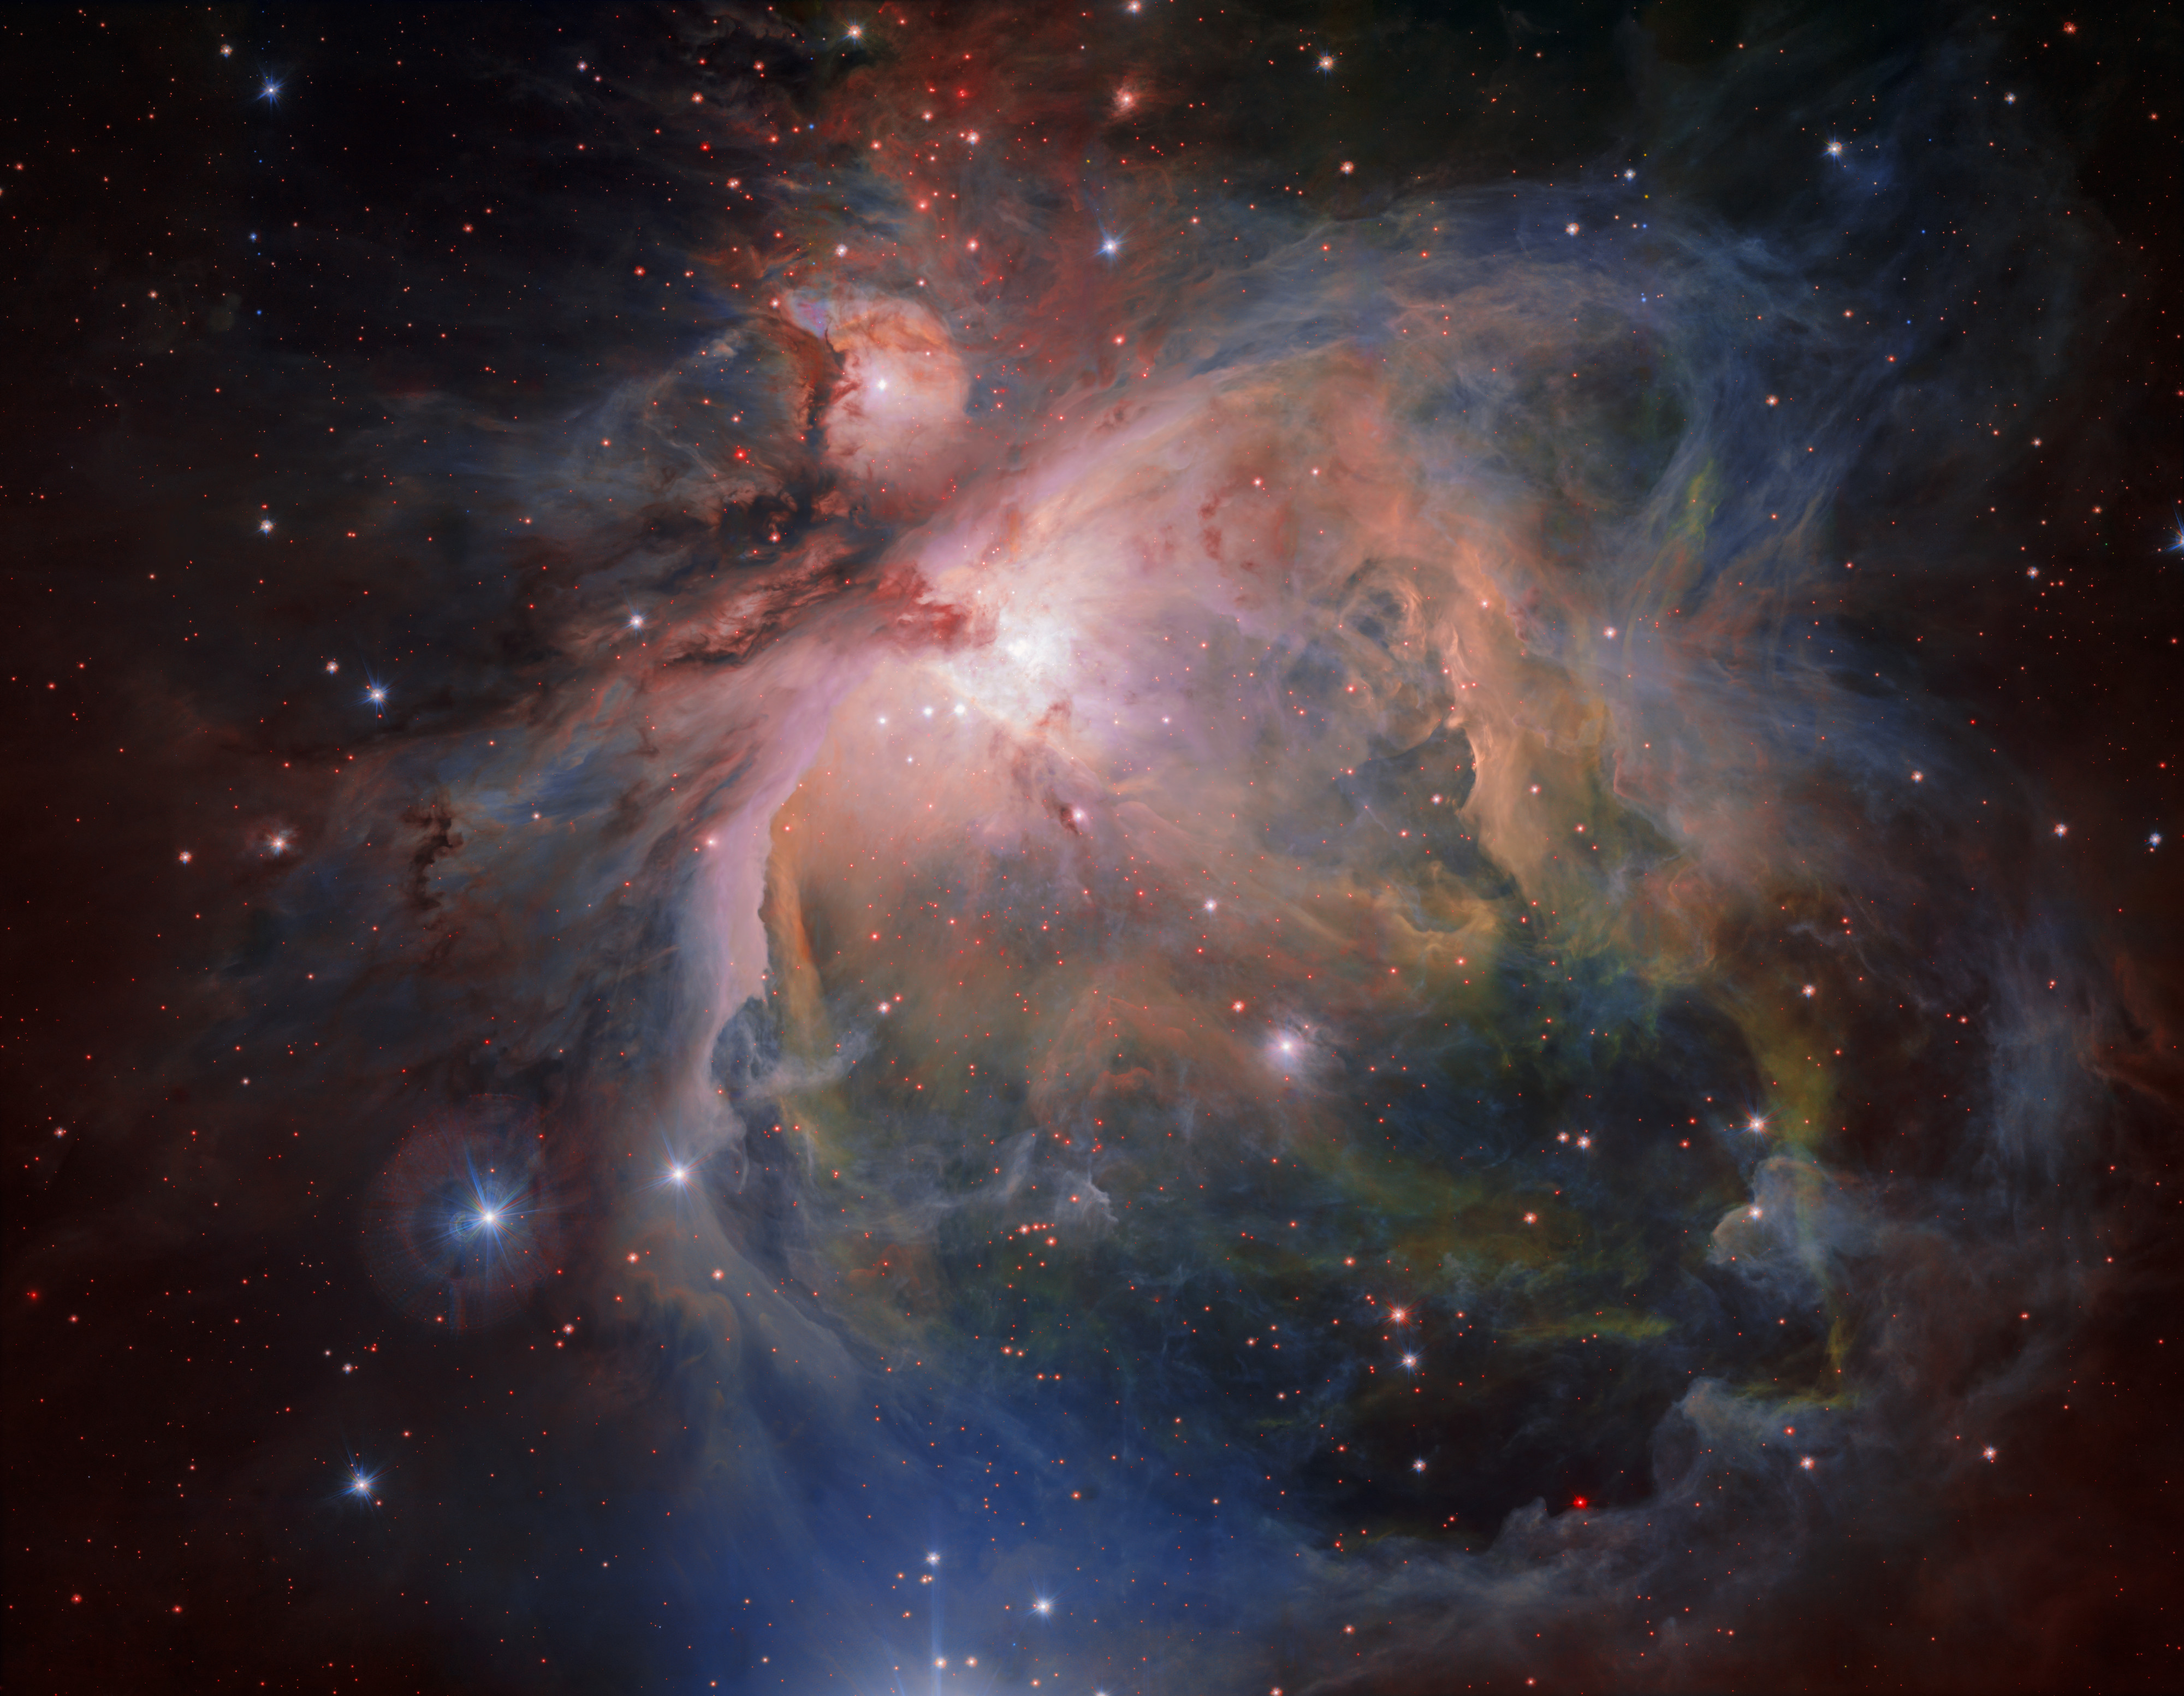
\includegraphics[width=0.40\textwidth]{./images/nebulosa-orione.jpg}
		\hspace{0.03\textwidth}
		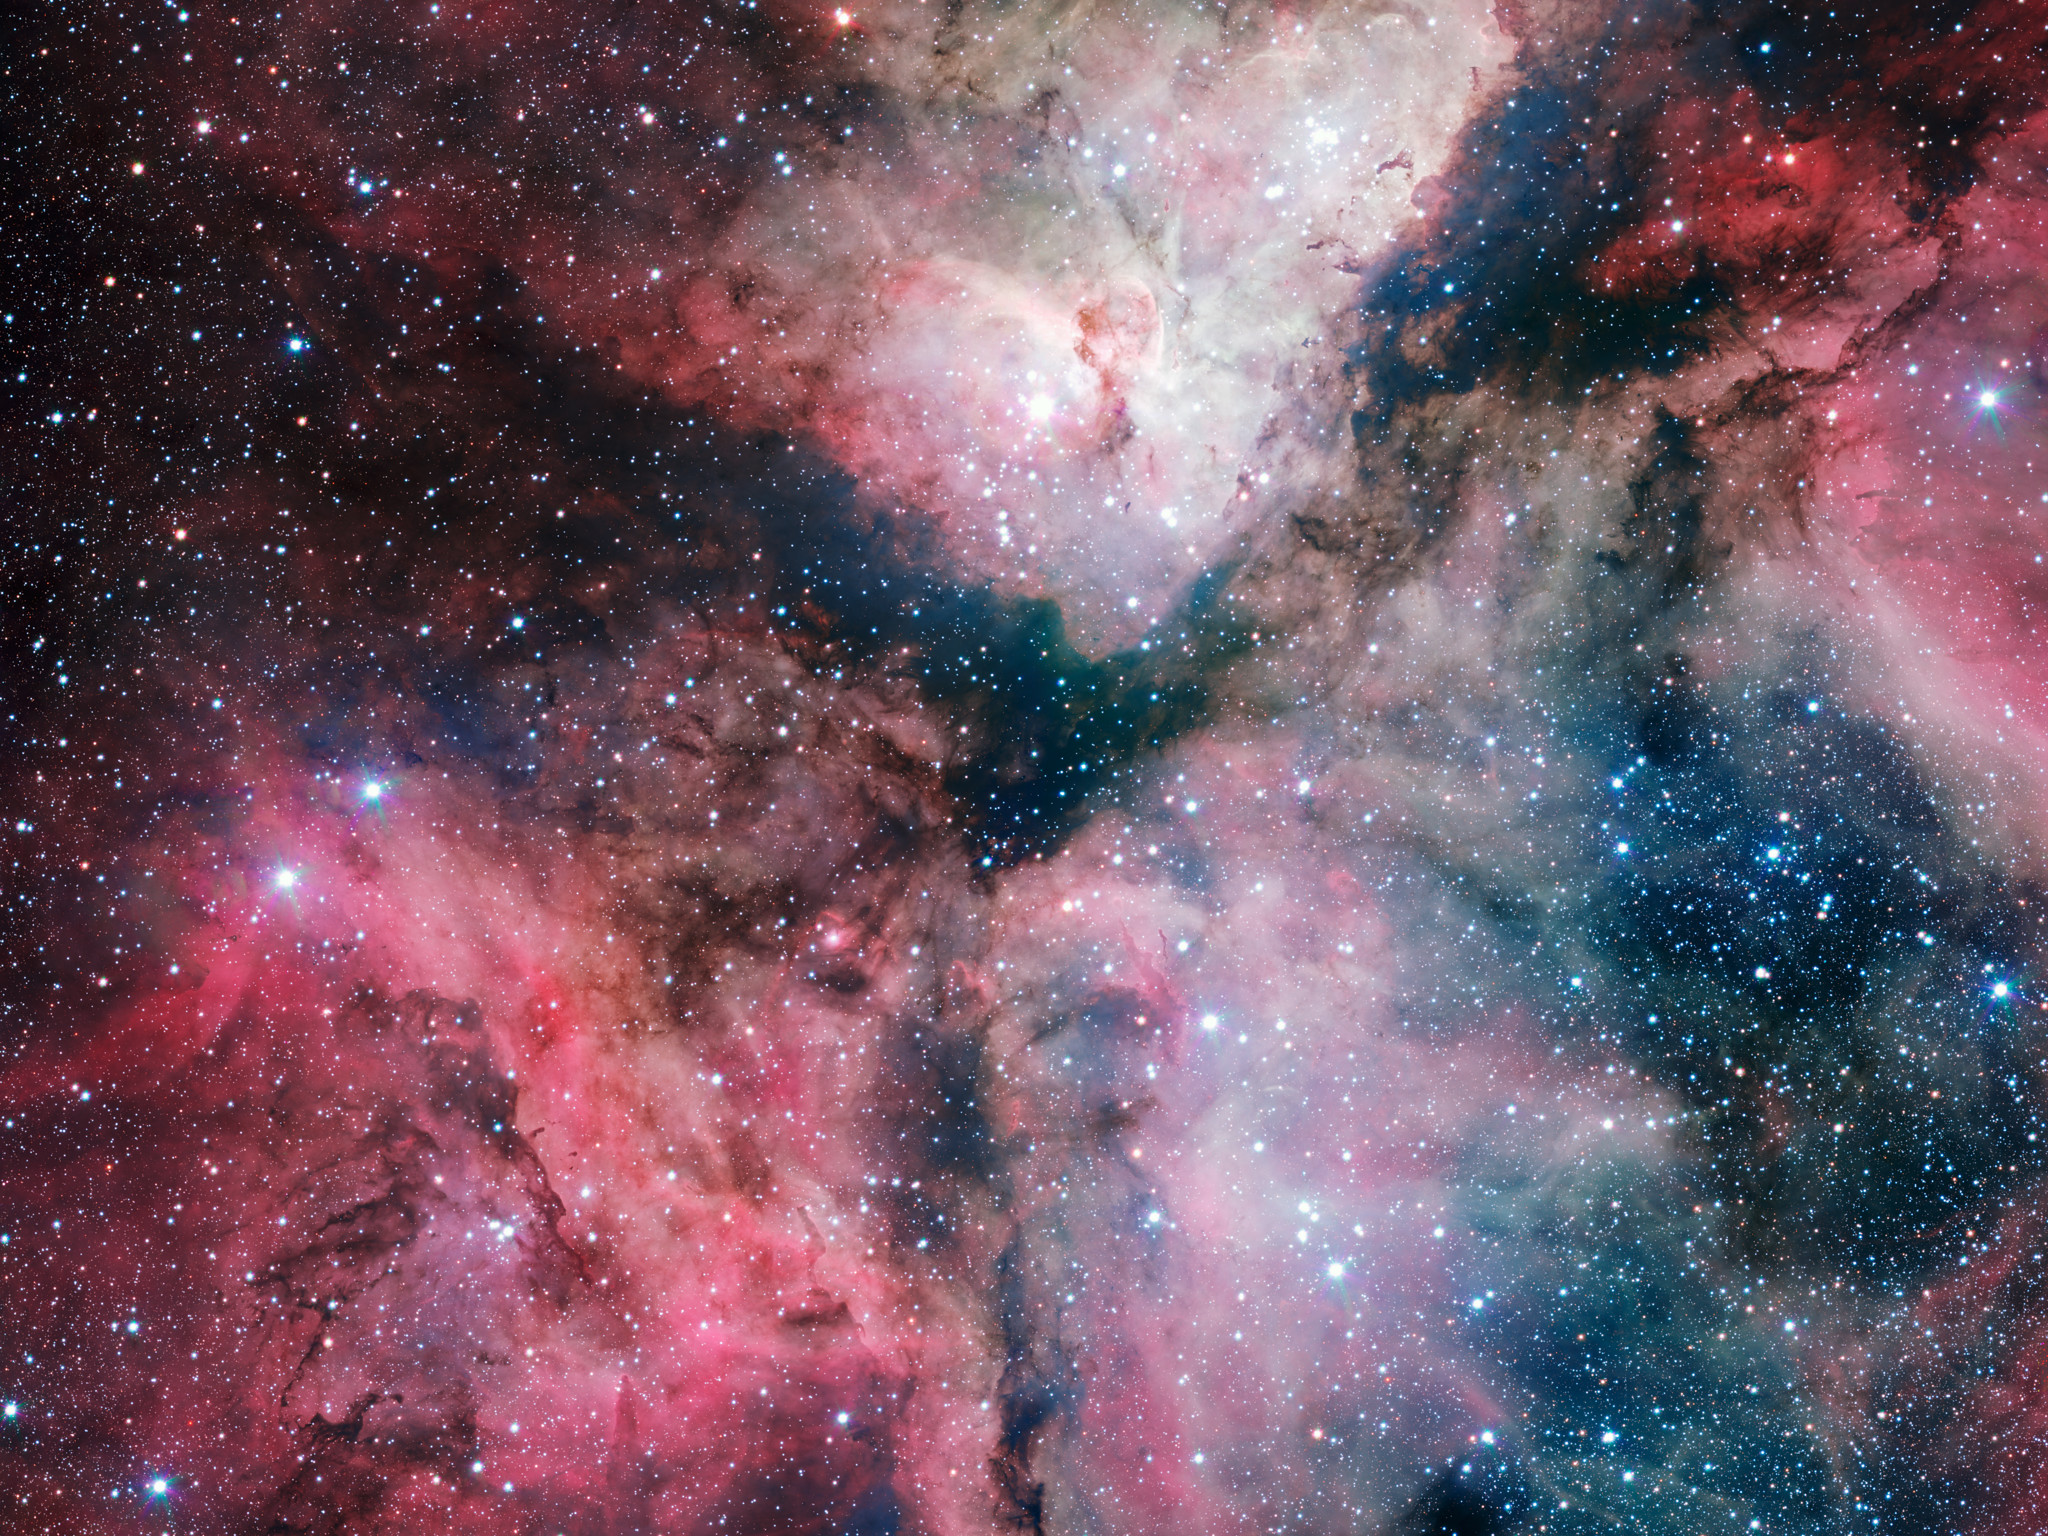
\includegraphics[width=0.41\textwidth]{./images/nebulosa-carena.jpg}
	}
	\caption{The Orion Nebula (left, credits: ESO/G. Beccari) and the Carina Nebula\\(right, credits: ESO; VPHAS+ Consortium/Cambridge Astronomical Survey Unit).}
	\label{fig:nebulose}
\end{figure}
\section{Stellar Clusters}
\label{sec:ammassi-stellari}
When numerous stars are born in the same region of space, they can remain gravitationally bound to one another, giving rise to self-gravitating systems known as stellar clusters.\\In these systems, each star contributes to the overall gravitational field and is continuously affected by the attraction exerted by all the other components \cite{krumholz2019}.
\begin{figure}[H]
	\centering
	\makebox[\textwidth][c]{
		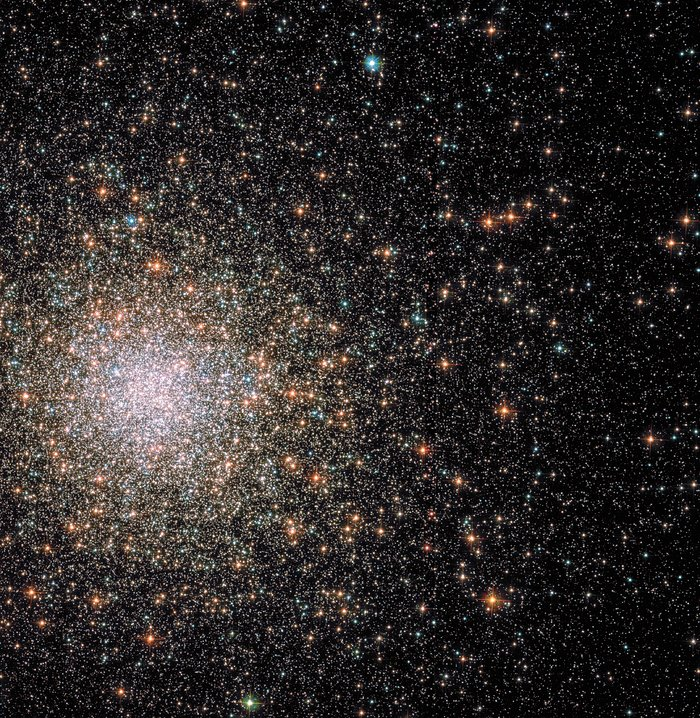
\includegraphics[width=0.29\textwidth]{./images/m62.jpg}
		\hspace{0.03\textwidth}
		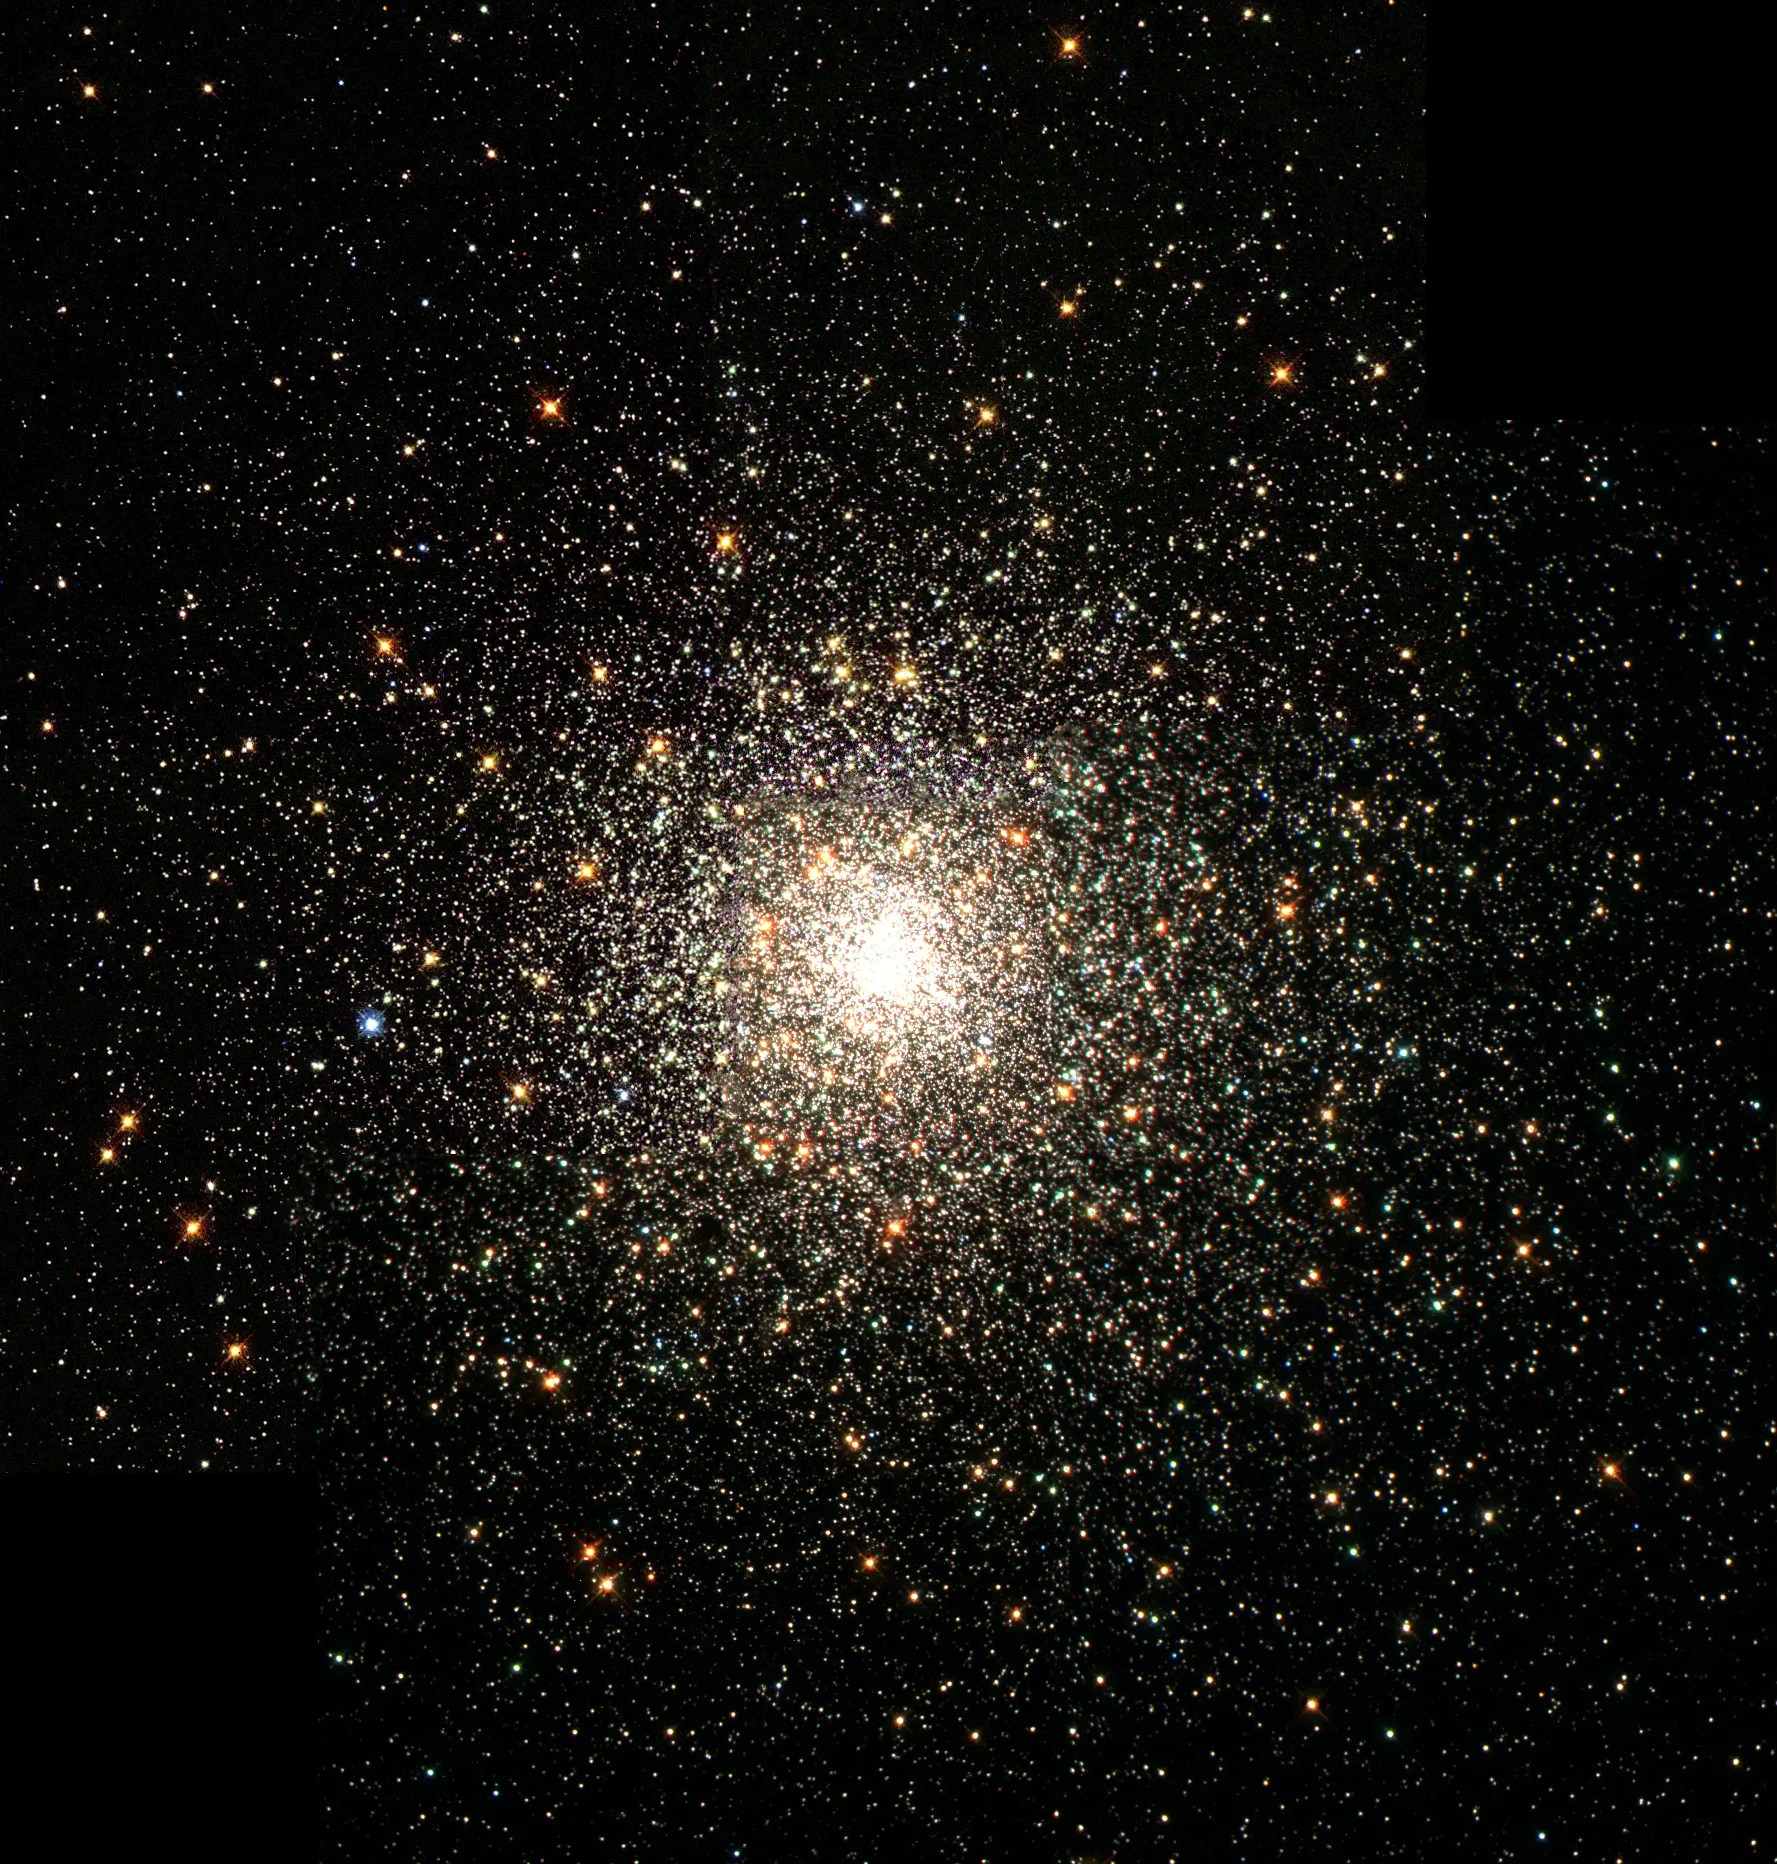
\includegraphics[width=0.285\textwidth]{./images/m80.jpg}
	}
	\caption{The globular clusters Messier 62 (left, credits: ESA/Hubble) and Messier 80\\(right, credits: NASA).}
	\label{fig:confronto-ammassi}
\end{figure}
\noindent These magnificent and imposing structures are particularly sensitive to gravitational interactions with their surrounding environment. The influence exerted by the galaxy that hosts them can profoundly alter their structure and compromise their delicate gravitational equilibrium.
\section{Galactic Tidal Stripping}
\label{sec:galactic-tidal-stripping}
As a stellar cluster orbits a galaxy, each of its stars experiences the galaxy's gravitational attraction to a different extent, depending on its position. These differences in the strength of gravitational attraction generate the so-called tidal forces, which can profoundly alter the cluster's equilibrium and evolution.
The progressive loss of stars caused by this phenomenon is known as galactic tidal stripping and, in the most extreme cases, can lead to the complete disruption of the cluster, accompanied by the formation of long stellar structures that follow the orbit of the original system, known as tidal tails \cite{baumgardt2003}.
\begin{figure}[H]
	\centering
	\makebox[\textwidth][c]{
		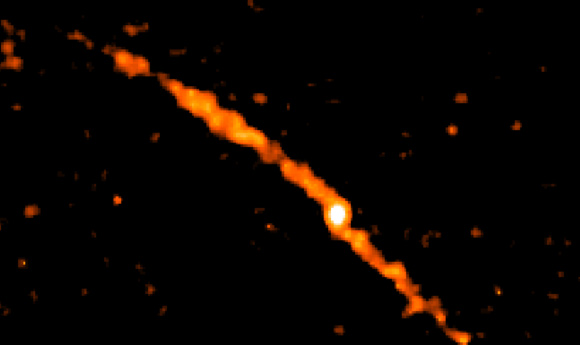
\includegraphics[width=0.40\textwidth]{./images/palomar5.jpg}
		\hspace{0.03\textwidth}
		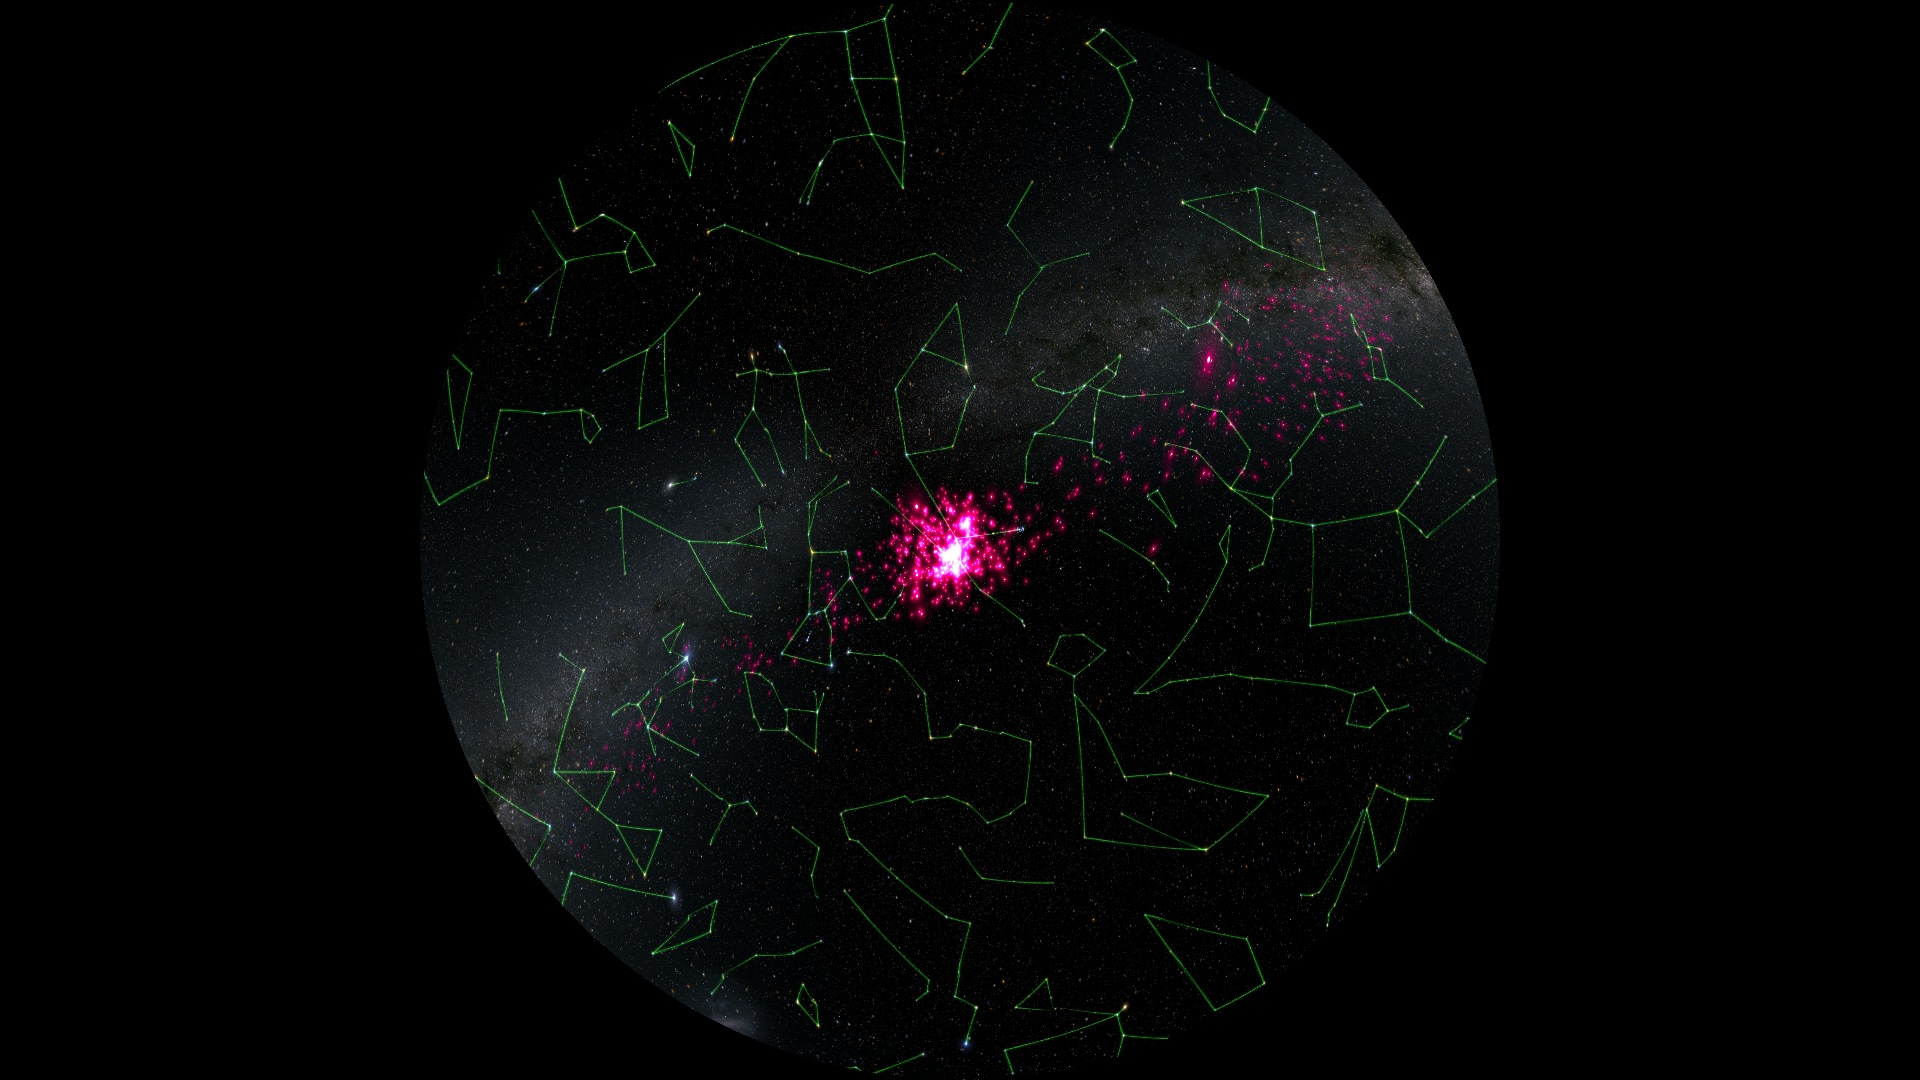
\includegraphics[width=0.42\textwidth]{./images/iadi.jpg}
	}
	\caption{Tidal tails of the globular cluster Palomar 5 (left, credits: SDSS) and a representation of the tidal tails of the Hyades open cluster, highlighted in pink (right, credits: ESA/Gaia/DPAC; S. Jordan/T. Sagrista).}
	\label{fig:code-mareali}
\end{figure}
\noindent Understanding the nature and intensity of this phenomenon is essential for studying the evolution and survival of stellar clusters. However, these processes unfold over extremely long timescales, which can span tens of millions of years.
\section{Computational Astrophysics}
\label{sec:astrofisica-computazionale}
Many astronomical phenomena unfold over timescales that cannot be directly followed through observations. To study them, modern astrophysics increasingly relies on mathematical models and computational tools. This approach, known as computational astrophysics, makes it possible to numerically reconstruct complex systems and analyse their evolution. A significant example is the \emph{Millennium Simulation}, which made it possible to study the formation of cosmic structures by tracking billions of dark matter particles \cite{springel2005}.
\section{Numerical Simulations}
\label{sec:simulazioni-numeriche}
To describe the evolution of a stellar cluster, each star can be represented as a particle with mass, position and velocity, and its motion can be calculated using the laws of gravity. This approach is known as an $N$-body simulation and makes it possible to numerically follow the interactions between all components of the system, also accounting for the influence of an external galactic gravitational force.
The main difficulty lies in the computational cost: in the direct summation method, the number of gravitational interactions to be calculated grows proportionally to the square of the number of stars in the system, quickly making the simulation of large systems computationally expensive. Simulating numerous initial configurations can therefore require considerable resources and time \cite{spurzem2023}.\\ This need has led to an interest in tools capable of using simulation results to make new predictions in a much shorter time.
\section{Machine Learning}
\label{sec:apprendimento-automatico}
Machine learning is a set of computational techniques that allows algorithms to learn relationships and recurring patterns from data. In astrophysics, it is used, among other applications, to classify celestial objects, analyse observations and build predictive models \cite{rodriguez2022}.
When applied to the results of numerical simulations, it makes it possible to learn the relationship between a system's initial conditions and its final behaviour. In this way, a trained model can provide estimates for new configurations without necessarily having to repeat the entire simulation each time, offering a complementary tool to traditional numerical methods.
\section{Objective}
\label{sec:obiettivo}
To study the evolution of stellar clusters subject to galactic tidal stripping, analysing how their initial orbital parameters influence their survival. To use the data obtained from simulations to train machine learning models, with the aim of predicting the final state of clusters from their initial orbital conditions and thereby reducing the computational cost required to obtain these estimates.%
